\documentclass[12pt]{article}
%\usepackage[utf8]{inputenc}
%\documentclass[UTF8]{ctexart}
%\usepackage[UTF8, heading = false, scheme = plain]{ctex}
\usepackage{geometry}
%geometry{a4paper,scale=0.9}
\geometry{a4paper,left=1cm,right=1cm,top=1cm,bottom=2cm}
\usepackage{amsfonts}
\usepackage{color}
\usepackage{url}
%\usepackage{biblatex}
\usepackage{amsmath}
\usepackage{amssymb}
\usepackage{latexsym}
\usepackage{cite}
%\addbibresource{ref.bib}
%\bibliography{ref.bib}
\usepackage{caption}
\usepackage{graphicx, subfig}
\usepackage{float}
%\usepackage[fontset=ubuntu]{ctex}
%\usepackage{fontspec}
\usepackage{xeCJK}
%\usepackage[colorlinks,
%anchorcolor=black,
%citecolor=black]{hyperref}
%\setmainfont{SimSun}
\usepackage[section]{placeins}
\usepackage{enumitem}
\usepackage{framed}
\usepackage[framemethod=TikZ]{mdframed}
\usepackage{indentfirst}
\usepackage{setspace}%使用间距宏包
\linespread{1.5}
%\title{预备知识}
%\author{leolinuxer }
%\date{June 2020}

\title{极大似然函数、最小二乘、交叉熵比较\cite{Comparison_Of_Maximum_Likelihood_Least_Square_Cross_Entropy}}
\author{leolinuxer}
%\date{June 2020}

\begin{document}
\maketitle
\tableofcontents

\section{似然函数}
\subsection{似然函数和概率密度函数的关系}
$$
L(\theta|x) = f(x|\theta)
$$

该公式表示给定联合样本$x$ 时,关于(未知)参数 $\theta$的函数。

其中$x$为随机变量$X$可以取到的值,即 $X=x$; $f(x|\theta)$ 表示给定 $\theta$ 值时,关于联合样本值$x$的联合密度函数(注:按照连密度函数的写法,$f(x|\theta)$应该写为$f(x,\theta)$【待验证】)。

\textbf{在此需要注意的是,似然函数与密度函数本是不同的数学对象: 前者是关于$\theta$的函数,后者是是关于随机变量 $x$的函数。仅仅是在此,两者的值相同。}

\subsection{与极大似然估计(MLE)的关系}
若x是离散随机变量,则有:
$$
f(x|\theta) = P_\theta(X = x)
$$
表示在参数 $\theta$下, $X$ 取 $x$ 的可能性大小。

并且若有
$$
L(\theta_1|x) = P_{\theta_1}(X=x) > L(\theta_2|x) = P_{\theta_2}(X=x)
$$
则可以认为 $\theta_1$ 比$\theta_2$ 要更接近真实值。

由此引出极大似然估计(MLE)。

\section{极大似然估计(MLE)}
\textbf{核心思想:通过最大化似然函数来获取最接近真实值的参数 $\theta$ 。}

举个典型的例子:已知口袋中有10个球,球可能是白色或黑色。每次抽取一个球,记录颜色后放回口袋。
如果抽取10次,白球出现7次,黑球出现3次,问口袋里最有可能的白球总数量。

我们会很自然的觉得白球很有可能是7个。
其中的思考过程即是极大似然估计的思想——认为观测到的情况总是在众多可能中最大概率发生的那一个。

将抽球结果作为离散随机变量$X$ ,设白球为 $X=1$,黑球为$X=0$ 。假设抽到白球的概率为 $\theta$ , $\theta$ 即是未知的需要通过极大似然估计得出的参数。
写出似然函数。
$$
L(\theta|x) = f(x|\theta) = P(x,\theta) = \theta^x \cdot (1 - \theta)^{1-x}
$$
抽到白球,则密度函数为$\theta$,抽到黑球则是$1-\theta$。

对于10次有放回抽球可以认为是10次独立事件,其\textbf{符合二项分布}。

对于二项分布,出现符合观测情况的,白球出现7次,黑球出现3次的概率密度函数为
$$
P(X,\theta) = P(x_1,\theta)\cdot P(x_2,\theta)\cdot \cdots \cdot P(x_{10},\theta) = \theta^7\cdot(1-\theta)^3
$$

写成似然函数形式为:
$$
L(\theta|x) = P(X,\theta) = \theta^7\cdot(1-\theta)^3
$$

此时可以清楚看到$\theta$是似然函数的自变量。那么当我们假定$\theta$为0.5时,可得似然函数值为0.0009765625,若假定 $\theta$为0.7时,似然函数值为0.1093543。后者要显然大于前者,因此我们认为白球占总数的70\%是更有可能发生的,因为这样\textbf{使得发生我们所观测到的现象的发生概率最大}。
\begin{figure}[H]
    \centering
    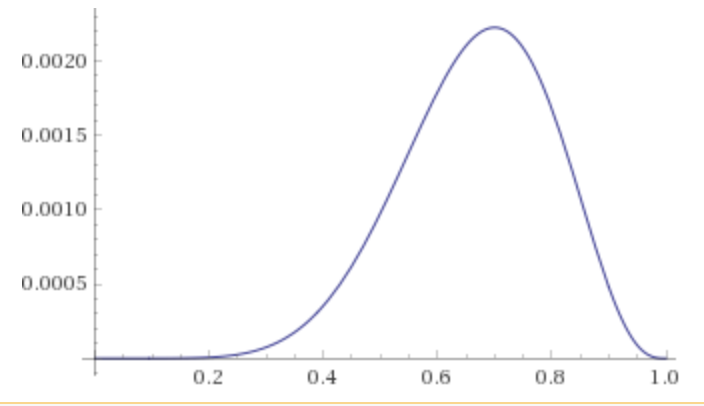
\includegraphics[width=.5\textwidth]{fig/likelihood_distribution_dice_example.png}
    \caption*{$L(\theta|x)$的图像,可以看出$x=0.7$时$L(\theta|x)$取得最大值}
\end{figure} 

我们可以通过对似然函数求导,来求得其极大值:
$$
\frac{dL}{d\theta} = 7\theta^6\cdot(1-\theta)^3 - \theta^7\cdot3\cdot(1-\theta)^2 = 0
$$
求得,当$\theta=0.7$ 时,似然函数取到极大值,因此我们认为白球占总数70\%时,10次抽球最可能出现7次白球。

\section{由极大似然估计推导最小二乘公式}
给定线性模型:$\hat{y} = wx$,可以认为观测值为$y = \hat{y} + \epsilon$,其中$\epsilon$为误差,其分布符合正态分布$\epsilon \sim N(0, \sigma^2)$,则观测值也同样符合正态分布,即:
$$
y \sim N(wx, \sigma^2)
$$

正态分布的密度函数为:
$$
f(x|w) = \frac{1}{\sqrt{2\pi}\sigma}e^{-\frac{(y_i - wx)^2}{2\sigma^2}}
$$

为了方便求极大值,我们对似然函数取对数,即\textbf{对数似然}:
$$
\ln{L(w|X)} = \sum_{i=1}^n\big[\ln{\frac{1}{\sqrt{2\pi}\sigma}} - \frac{(y_i - wx)^2}{2\sigma^2}\big]
$$

其中$\sigma$为常数,\textbf{则当$\frac{(y_i - wx)^2}{2\sigma^2}$取得最小时,对数似然取得最大,也即似然函数取得最大。而后者即是最小二乘法所用的均方误差公式,在整个最小二乘过程中,都在试图使其降低,其结果也就是使得似然函数极大。}

\section{极大似然估计推导交叉熵}
\subsection{二分类问题}
二分类模型可认为符合二项分布,设$X=\{0,1\}$, $y$ 为样品的真实类别。则有:
$$
P(X=0,w) = 1 - P(X=1,w)
$$

因此有:
$$
f(x|w) = [P(X=1,w)]^y\cdot[1 - P(X=1,w)]^{1-y}
$$

对于$m$次观察结果,则有:
$$
f(X|w) = \prod_{i=1}^m\{[P(X=1,w)]^y\cdot[1 - P(X=1,w)]^{1-y}\}
$$

写出似然函数并取对数形式,则有:
$$
\ln{L(w|X)} = \ln{f(X|w)} = \sum_{i=1}^m\big[y_i\ln(P(X=1,w)) +  (1-y_i)\ln(1-P(X=1,w))\big]
$$

当$ -\big[y_i\ln(P(X=1,w)) + (1-y_i)\ln(1-P(X=1,w))\big]$ 取得最大时,则似然函数也取得最大。

通常我们做二分类时,最后通过sigmoid激活函数输出,其输出值即是$\hat{y} = P(X=1|w)$。
因此将上式化简,即是binary cross entropy形式:
$$
-\big[y\ln(\hat{y}) + (1-y)\ln(1-\hat{y})\big]
$$

\subsection{多分类问题}
多分类问题将二项分布扩展到多项分布,设有$n$个类别,则有:
$$
f(X|w) = \prod_{C=1}^nP(X=C,w)^{y_C}
$$

同样的,对于$m$个样本,写出其对数似然:

(【原文疑似有误,原文为】)
$$
\ln{L(w|X)} = \sum_{i=1}^m[(1-x_i)\sum_{C=1}^n y_{iC}\ln{P(X=C,w)}]
$$

(【原文疑似有误,自己推导为】)
$$
\ln{L(w|X)} = \sum_{C=1}^n y_{iC}\ln{P(X=C,w)}
$$

其中$- \sum_{C=1}^n y_{iC}\ln{P(X=C,w)}$即是cross entropy,当其取得最小时,似然函数取得最大。

\section{总结}
可以看到机器学习中常见的三个损失函数:mean square loss, binary cross entropy loss, categories cross entropy loss,其背后的原理都指向了极大似然估计。可见损失函数的定义并不是简单的“衡量预测值与真实值的距离
”,其背后有着严谨的数学在为其可靠性做担保。

\bibliography{../ref}
\bibliographystyle{IEEEtran}
\end{document}
